\section{Introduction}
\label{hilo:sec:introduction}

Chapter~3 opens the visual-understanding part of the thesis by studying how learning can reflect the relational structure of a scene when predicate annotations are long-tailed and semantically overlapping. A vocabulary of $56$ predicates makes the label space explicit, but standard empirical risk minimization still allows frequent predicates to dominate the learned representation. The resulting model captures only a biased projection of the annotated graph structure.
The goal of this chapter is therefore to establish a strong closed-set PSG formulation that recovers both common and rare predicates. HiLo makes the head--tail organization of the predicate space operational through complementary branches and consistency constraints, before the later chapters incorporate language-derived structure and open-set capability.

Scene Graph Generation (SGG)~\citep{lu2016visual} is a crucial task in image scene understanding that extracts triplets in the form of subjects, objects and their relations to build a scene graph. 
Subjects and objects are represented with bounding boxes.
Since this task links vision and text, it holds great potential for a variety of applications, including visual question answering \citep{hildebrandt2020scene}, image captioning \citep{gao2018image, chen2020say}, image retrieval \citep{johnson2015image, schuster2015generating, qi2017online} and visual reasoning \citep{aditya2018image, shi2019explainable}.

Recently a novel variant of SGG was proposed, which is Panoptic Scene Graph generation (PSG) \citep{yang2022panoptic}.
Subjects and objects are represented with panoptic segmentation~\citep{kirillov2019panoptic} masks. Unless stated otherwise, the visual understanding chapters of this thesis focus on PSG, since it is pixel-level accurate and also covers background classes and their relations with foreground objects.

The performance of the PSG model is affected by a \emph{long-tail problem} in its relation categories.
For instance, relations such as \textit{over}, \textit{in front of} and \textit{holding} occur tens of thousands of times in the PSG dataset~\citep{yang2022panoptic}, while others like \textit{swinging} and \textit{kissing} occur only a few dozen times.
This severe class imbalance in the relation categories can lead to model predictions that are more inclined to high-frequency relations, which poses significant challenges to the application of panoptic scene graphs in real-world scenarios.

Previous methods \citep{chiou2021recovering, desai2021learning, li2021bipartite, deng2022hierarchical} have often treated the long-tail problem of the PSG task as equivalent to the long-tail problem in object-centric tasks such as classification \citep{cui2019class, cao2019learning, hong2021disentangling} or semantic segmentation \citep{cui2022region, alexandridis2022long}.
Consequently, these methods have employed re-balancing techniques to address class imbalance, either through re-sampling the data \citep{li2021bipartite} or by using a class-balanced loss~\citep{kang2023skew} that assigns different weights to different relation categories.

In contrast, in the relation-centric PSG task, a subject-object pair can have multiple relations that exhibit \textit{relational semantic overlap}, such as being partially or fully overlapping.
For example, in Fig.~\ref{hilo:fig:motivation}, there are multiple relations between the boy and the sports ball, such as \textit{beside}, \textit{looking at}, \textit{playing} and \textit{chasing}.
%
%PSG methods can be considered as either biased (following the natural distribution) or unbiased (taking special measures to re-balance the distribution).
For regular biased models \citep{xu2017scene, zellers2018neural, tang2019learning, lin2020gps}, the results are dominated by high-frequency relations (\textit{beside}, \textit{looking at}).
%
For specifically unbiased models \citep{zhang2022fine, yang2022panoptic}, the results are dominated by low-frequency relations (\textit{playing}, \textit{chasing}).
%
However, since the low frequency relations can be more specific (\eg \textit{on} and \textit{standing on}) or only partially overlapping with high frequency relations (\eg \textit{looking at} and \textit{chasing}), it is crucial to include both to fully understand the image.
%
We found that relational semantic overlap occurs in large numbers in the PSG dataset~\citep{yang2022panoptic} and that current methods do not effectively address it.
This is reflected in the increase in the category-averaged \textit{mean recall} metric of unbiased methods, at the cost of the decrease in global \textit{recall} (see Sec.~\ref{hilo:sec:experiments:main_results}).


\begin{figure}
\centering
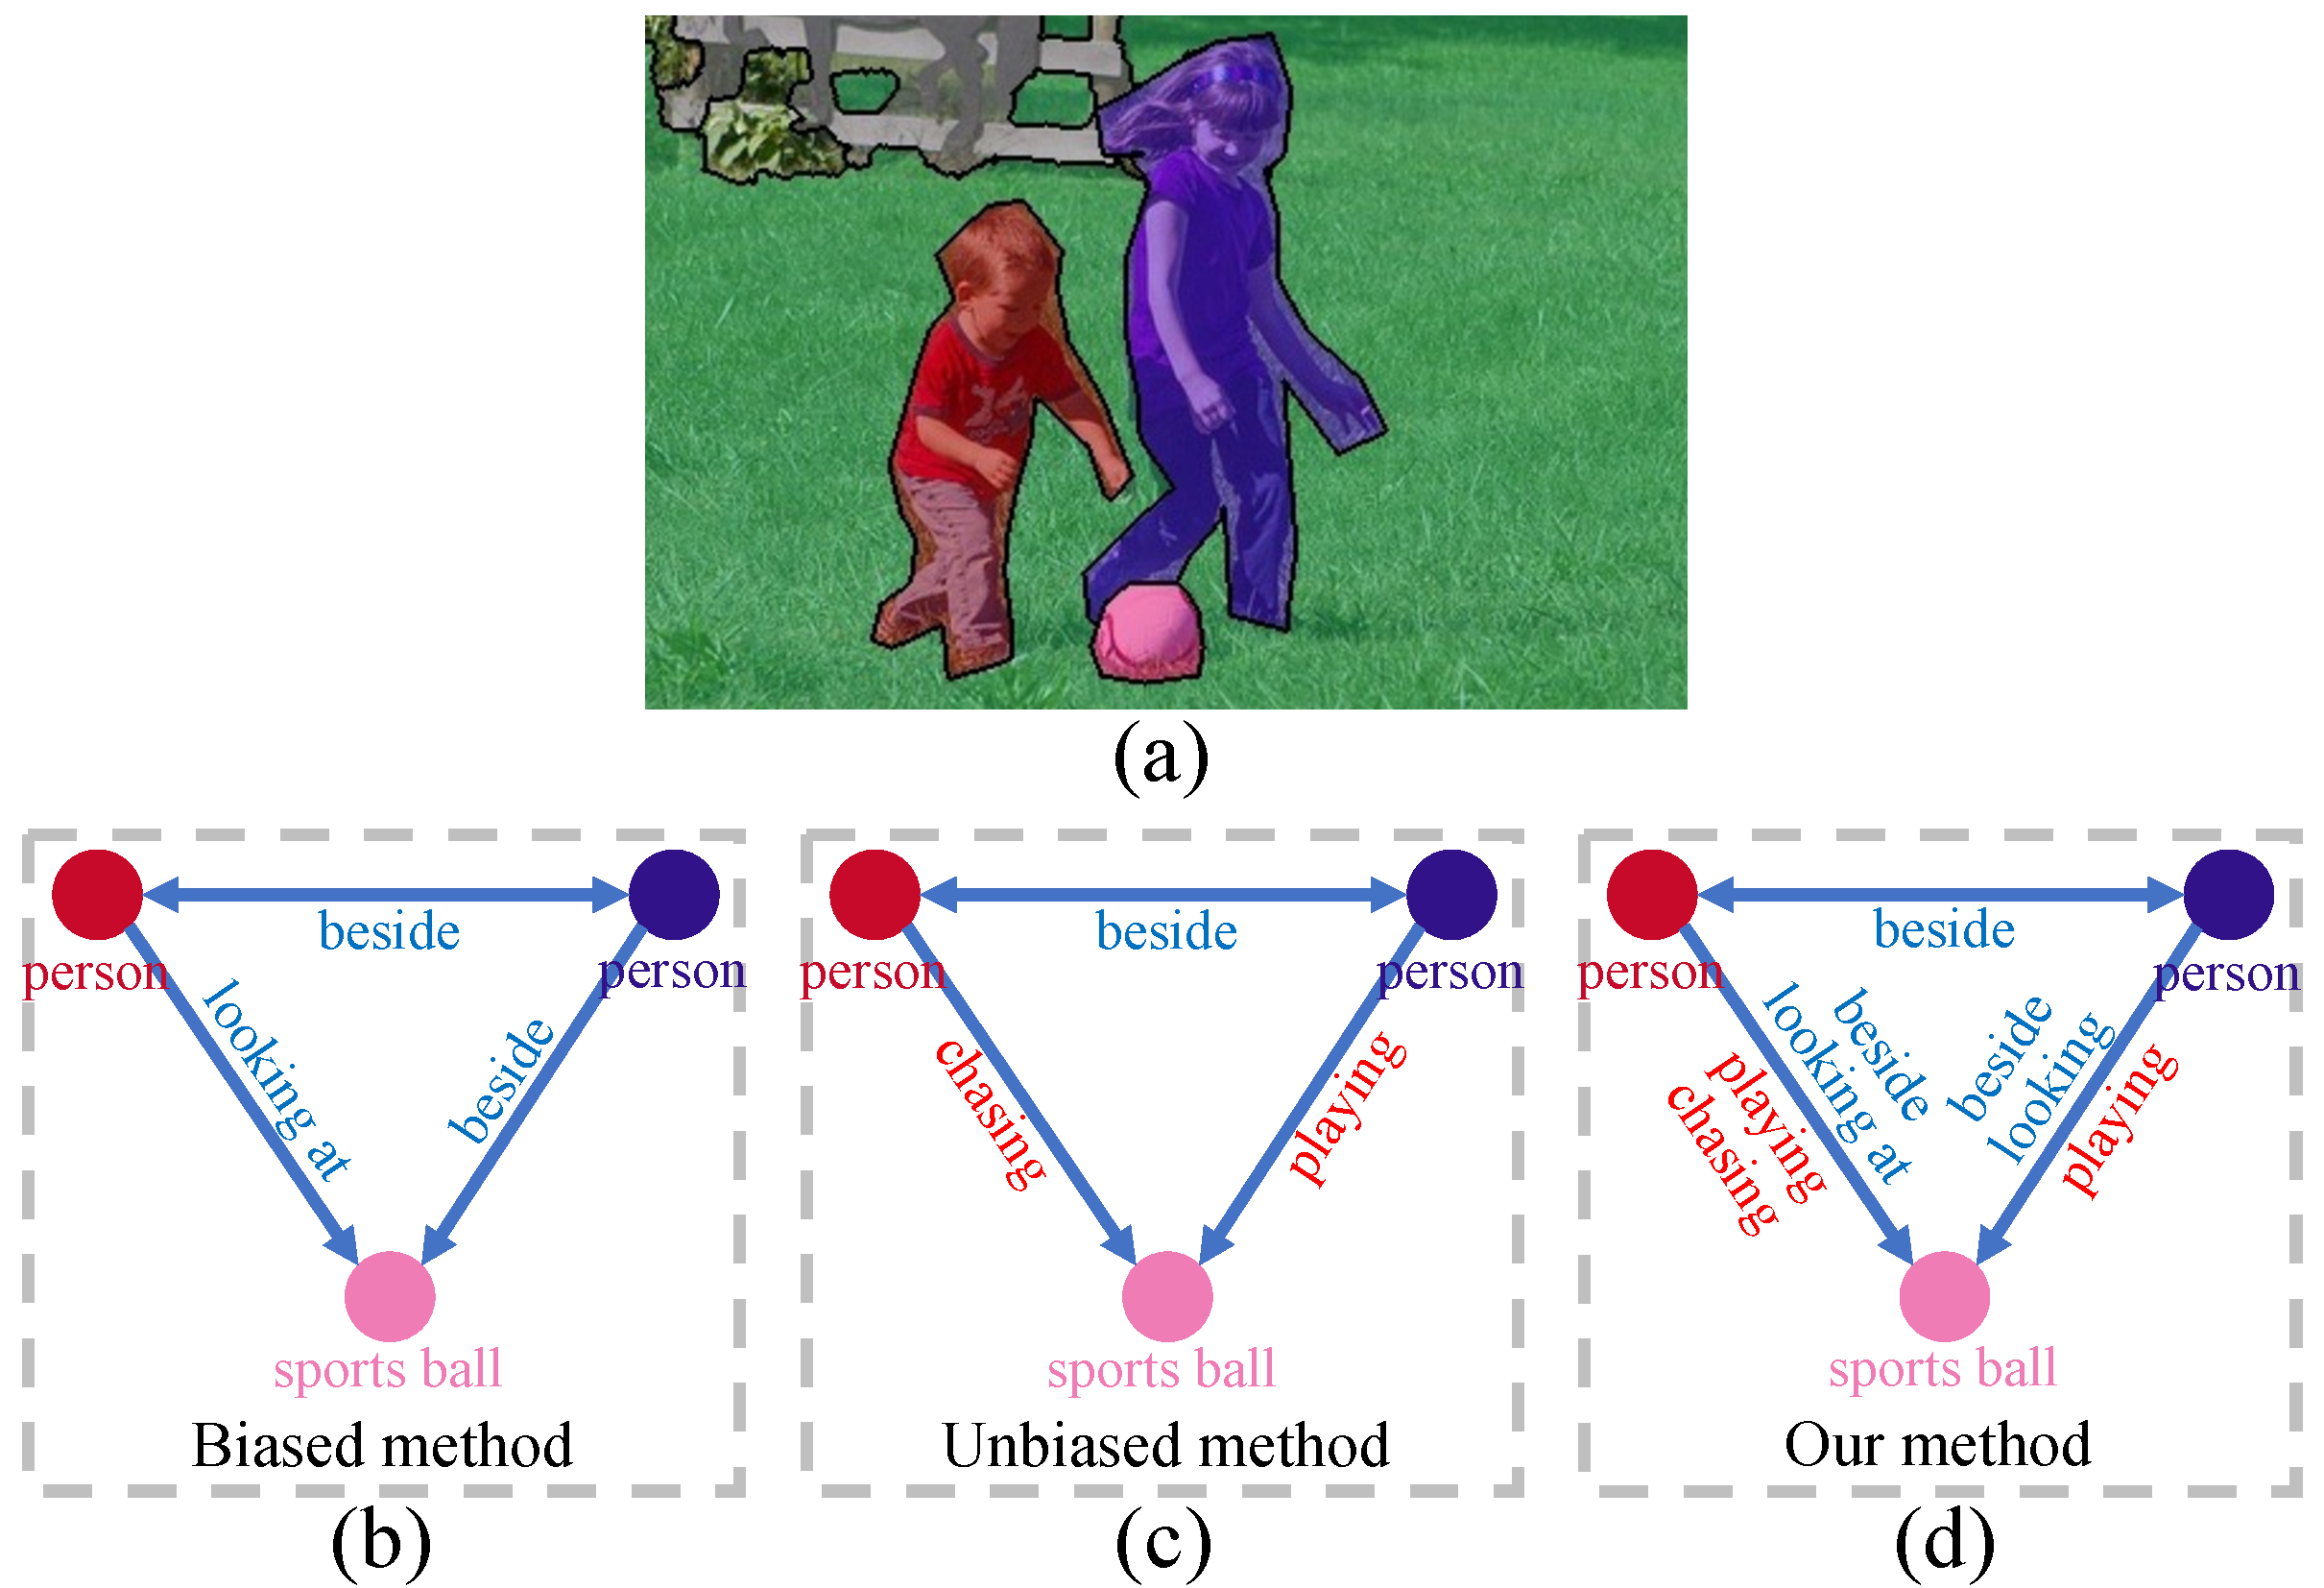
\includegraphics[width=0.7\textwidth]{Chapter3/Figures/motivation}
\caption{
An example of the PSG task. We compare the predicted object relations of different approaches. 
a) An image and its panoptic segmentation. Two persons and a sports ball are shown in different colors.
b) A biased method predicts mostly high frequency relations.
c) An unbiased method predicts mostly low frequency relations.
d) Our method predicts both low and high frequency relations, as well as more relations in total.
}
\label{hilo:fig:motivation}
\end{figure}


To address the long-tail problem of scene graphs under relational semantic overlap, we introduce the HiLo framework. This framework simultaneously learns the high and low frequency relations in different network branches and unifies their strengths with the help of two novel consistency loss functions.
%
We apply our framework on top of a novel baseline. This baseline uses a recent transformer-based approach~\citep{cheng2022masked} for panoptic segmentation and adapts triplet queries~\citep{yang2022panoptic} and masked attention~\citep{cheng2022masked} for the PSG task.
%
In summary, we make the following contributions:
\begin{itemize}
    \item We identify the long-tail problem with relational semantic overlap in the PSG task and propose the HiLo framework to address this problem. The framework is general and can be applied to any PSG method.

    \item We propose a powerful and efficient one-stage end-to-end baseline. This baseline enhances the interaction between mask and relation prediction in the transformer decoder layer.

    \item We conduct extensive experiments to demonstrate the effectiveness of our framework and baseline.
    Our results outperform the state-of-the-art in both recall and mean recall on the PSG dataset and show systematic improvements on the VG dataset.
\end{itemize}

Together, these results establish the first step of the PSG arc in this thesis.
Chapter~4 builds on this closed-set foundation by incorporating language information from large language models to further improve rare and ambiguous relation prediction.
